% !TEX encoding = UTF-8
% !TEX TS-program = pdflatex
% !TEX root = ../tesi.tex

%**************************************************************
\chapter{Progettazione}
\label{cap:progettazione}
\label{sec:tecnologie-strumenti}

In questo capitolo vengono illustrate le strategie di progettazione adottate per la realizzazione del prodotto in questione. La progettazione viene descritta ad alto livello senza descrivere in dettaglio tutti i diagrammi delle classi. 

\section{Progettazione Frontend}
\label{sec:progettazione}

\subsection{Atomic design}
Creata da Brad Frost nel 2013, l'Atomic design è una metodologia composta da 5 differenti fasi, utile per creare un sistema di interfacce in maniera gerarchica.
\begin{figure}[!h] 
	\centering 
	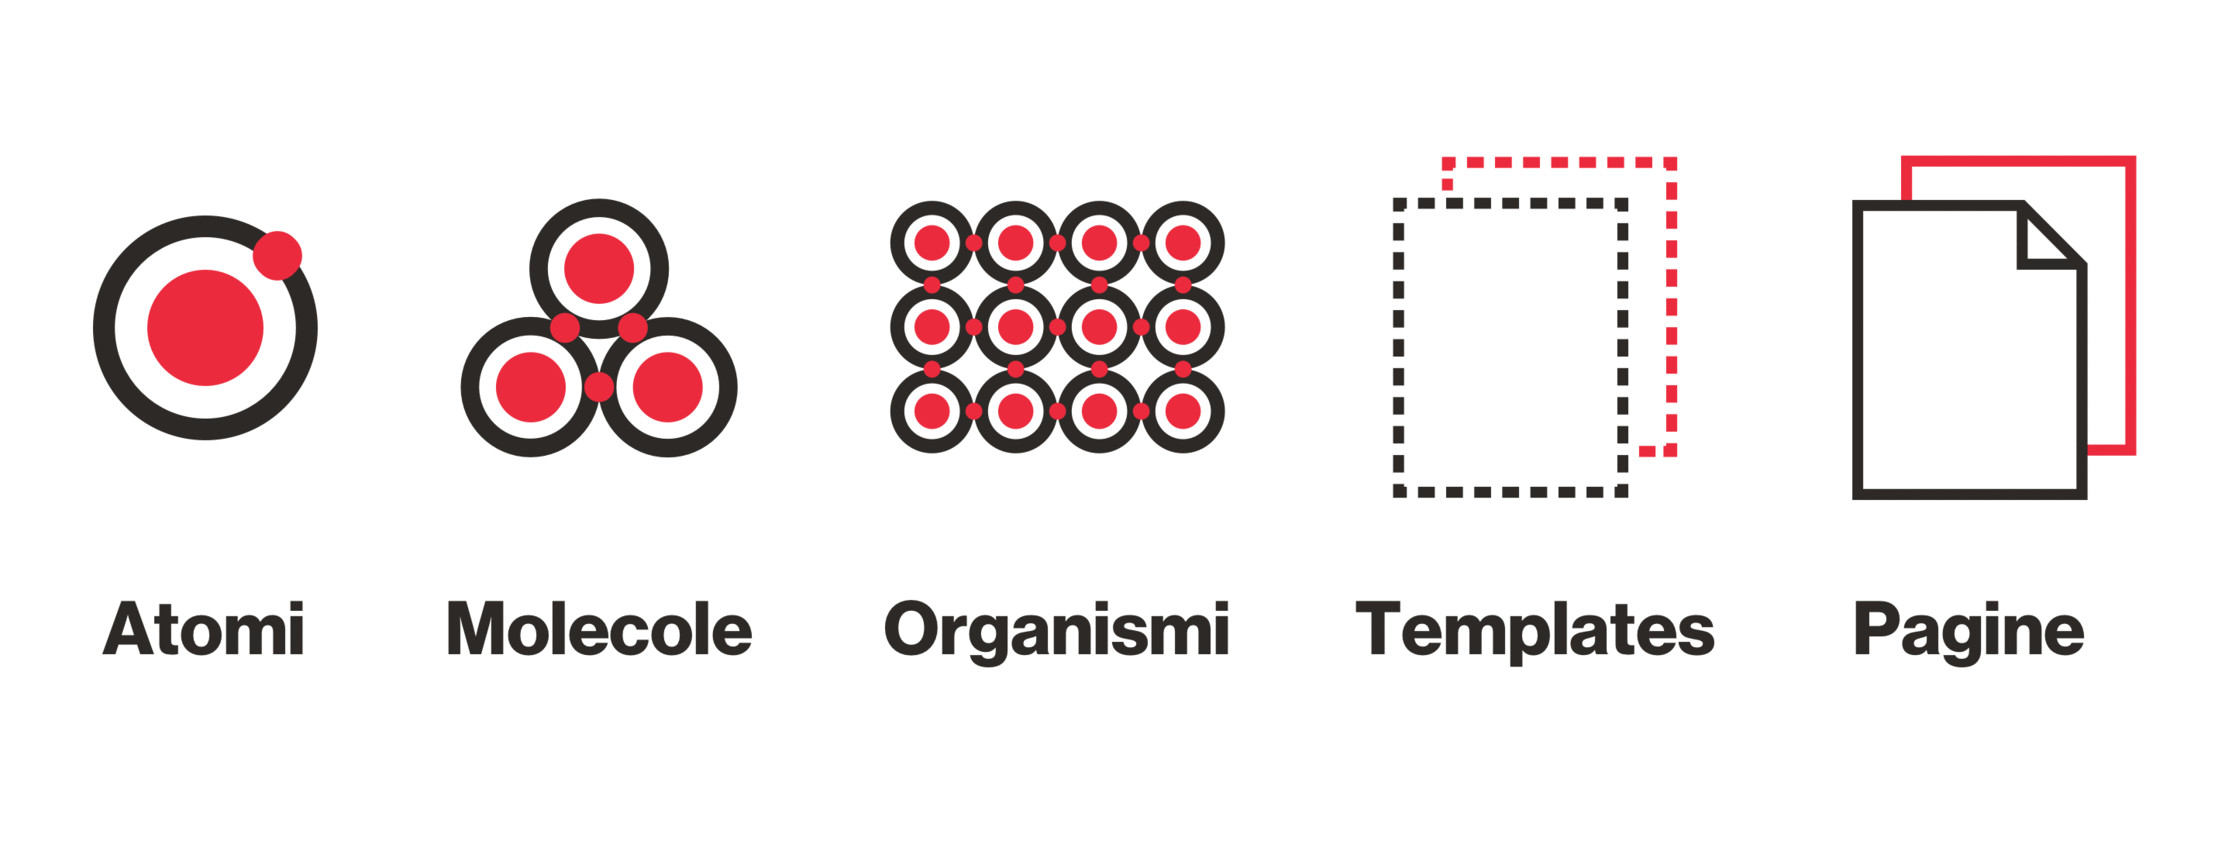
\includegraphics[width=0.8\columnwidth]{atomic} 
	\caption{Elementi atomic design}
\end{figure}
\\

\textbf{Atomi:} in fisica un atomo è la più piccola particella di un elemento che non subisce alterazioni nelle trasformazioni chimiche; nell’Atomic Design gli atomi sono i blocchi fondamentali che comprendono tutta l’interfaccia.
Questi atomi comprendono elementi HTML come tipografia, palette colori, input, bottoni e altri elementi che non possono essere suddivisi ulteriormente senza cessare di essere funzionali.
\\

\textbf{Molecole:} sono semplici gruppi di elementi d'interfaccia che funzionano uniti. Quando combiniamo due oppure più atomi, creiamo quindi una molecola.
\\

Nel contesto della applicazione gli atomi e le molecole sono rappresentate dai elementi della libreria Angular Material, che successivamente sono utilizzate per realizzare l'interfaccia di intera applicazione.

\begin{figure}[!h] 
	\centering 
	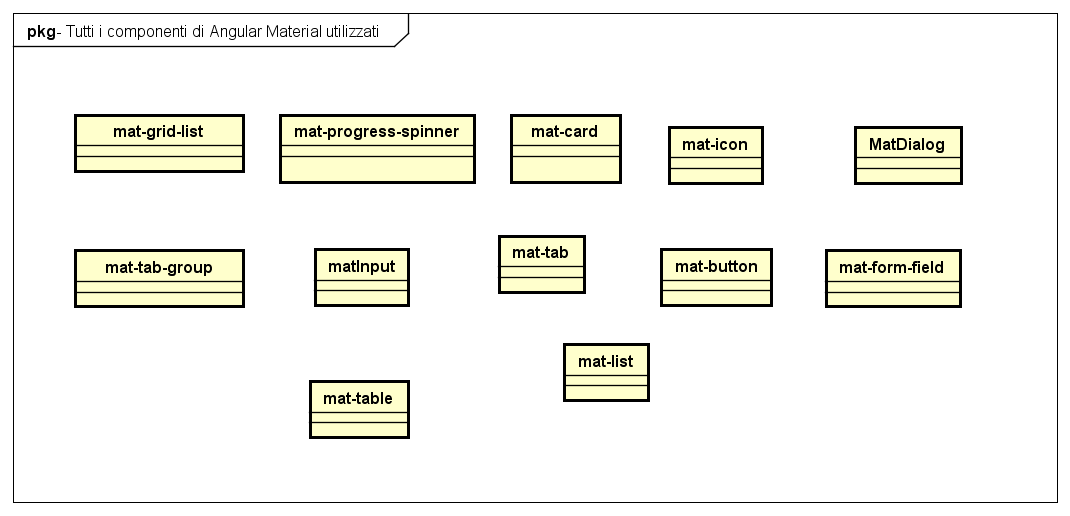
\includegraphics[width=1\columnwidth]{prog/angular} 
	\caption{Componenti Angular Material che formano gli atomi e le molecole dell'applicazione}
\end{figure} 

\textbf{Gli organismi} sono dei componenti più o meno complessi, composti da gruppi di molecole e/o atomi e/o altri organismi. Questi organismi creano diverse sezioni all'interno della nostra interfaccia. Un esempio può essere un menu di navigazione, che è formato in media da diversi pulsanti/link. 
\\

\textbf{I templates} sono creati dall'insieme dai nostri atomi, molecole e organismi. Creando così la prima idea di scheletro della pagina.
\\

\textbf{Le pagine} sono dei templates riempiti di contenuto reale, come immagini, testi, elementi grafici, advertising, ecc. Questo ci aiuta a capire come la pagina, a seconda del caso specifico, si comporterà quando il contenuto andrà a popolarla. 
\subsubsection{Namespace 1} %**************************
Descrizione namespace 1.

\begin{namespacedesc}
    \classdesc{Classe 1}{Descrizione classe 1}
    \classdesc{Classe 2}{Descrizione classe 2}
\end{namespacedesc}


%**************************************************************
\section{Design Pattern utilizzati}

%**************************************************************
\section{Codifica}
